\documentclass[dvipsnames,tikz]{standalone}
\usepackage{amsmath}
\usepackage{arevmath}
\usepackage{xcolor}
\usepackage{tikz}
\usetikzlibrary{calc}
\usetikzlibrary{decorations.pathreplacing,calligraphy,3d}

\tikzset{main/.style={draw=black, circle, color=black}}

\begin{document}
	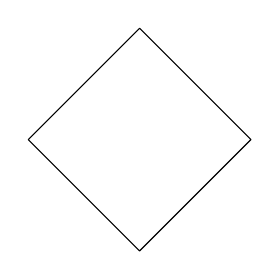
\begin{tikzpicture}[scale=1, main, line join=bevel]
		\draw[rotate=45] (-1,-1) rectangle (1,1);
	\end{tikzpicture}

	\foreach \n in {1,...,11}{%
		\begin{tikzpicture}[scale=1, main, line join=bevel]
			\draw[rotate=45] (-1,-1) rectangle (1,1);
			\foreach \a in {1,...,\n}{%
				\draw[rotate={(\a+1)*45}, scale=0.707^\a] (-1,-1) rectangle (1,1);
			}
		\end{tikzpicture}
	}
\end{document}